\section{\ExercisePrefixEmbeddedC Joysticks abfragen \optional}
Nachdem du im letzten Kapitel kennengelernt hast, wie du Texte und Zahlen auf dem Display ausgeben kannst, möchten wir in diesem Abschnitt diese Funktionen nutzen, um die analogen Werte der Joysticks auszugeben. Darauf aufbauend soll eine Funktion entwickelt werden, welche mithilfe des Joysticks die Farbe der RGB-LED verändern soll. Die zu implementierenden Funktionen für diesen Abschnitt befinden sich in der Datei joystick.c. Solltest du die Funktion writeText noch nicht implementiert haben, kannst du auf die Musterlösung zugreifen, da diese zur Ausgabe von Informationen in dieser Aufgabe benötigt wird. 
\begin{figure}
	\begin{centering}
		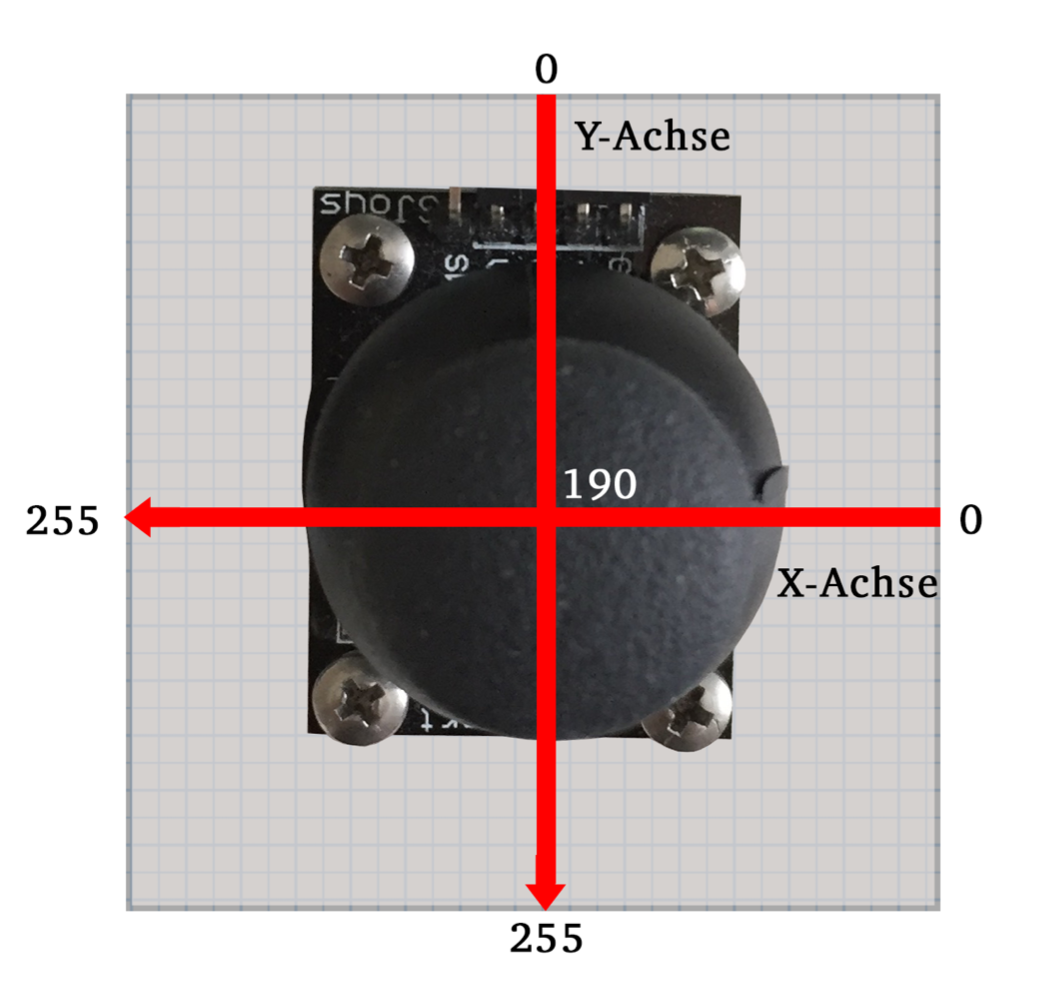
\includegraphics[width=.4\textwidth]{./05_c/figures/joystickValues.png}
		\caption{Wertebereich der Joysticks}
		\label{fig:jostickValues}
	\end{centering}
\end{figure}
\subsection{Analoge Werte auf dem Display anzeigen}

Jeder Joystick besitzt zwei analoge Leitungen, welche die X- oder Y-Position des Steuerknüppels auslesen. Die analogen X- und Y-Leitungen der Joysticks geben die Spannung der jeweils zwei Drehpotentiometer aus, welche zwischen 0 und 5V liegen und die Position des Joysticks angeben. Die Spannungswerte der Joysticks können durch den Analog-Digital-Wandler des Microcontrollers 8-Bit genau bestimmt werden und haben somit einen Wertebereich von 0 bis 255. Die Orientierung des Wertebereiches in X- und Y-Richtung ist in Abbildung \ref{fig:jostickValues} dargestellt. Durch Messungen der Werte für die X- und Y-Position des Joysticks wurde deutlich, dass dessen Wertebereich nicht gleich- mäßig verteilt ist, sondern die mittlere Position (190,190) ist. Die Ausrichtung der X- und Y-Achse sind entgegengesetz des kartesischen Diagramms ausgerichten. Joystick 1 ist mit den analogen Anschlüssen AN16 und AN19 und Joystick 2 ist mit AN13 und AN23 verbunden. 

(1.) Schreibe die Funktion printValues, welche über Zeiger auf die anlaogen Leitungen 13, 16, 19 und 23 die Werte der Joysticks ausliest und diese auf dem Bildschirm ausgibt. 

\begin{table}[]
	\centering
	\caption{Wichtige Funktionen und Variablen für das Joystick}
	\label{joystickInfo}
	\begin{tabular}{|l|l|}
	\hline
	\textbf{Funktionen/Variablen} & \textbf{Beschreibung} \\ \hline
	void setCursor(480,320) & Setzt den Cursor auf den Anfang \\ \hline
	void writeTextln(char{[}{]} text) & Schreibt text auf das Display und verschiebt den Cursor mit Zeilensprung \\ \hline
	void writeText(char{[}{]} text) & Schreibt text auf das Display und verschiebt den Cursor ohne Zeilensprung \\ \hline
	write3Digits16Bit(uint16\_t *number) & Schreibt eine Zahl an der Position des Curors auf das Display und verschiebt den Cursor weiter \\ \hline
	uint\_8 analog19 & Zeiger auf den Analogen-Kanal der X-Achse des Joysticks 1 \\ \hline
	uint\_8 analog16 & Zeiger auf den Analogen-Kanal der Y-Achse des Joysticks 1 \\ \hline
	uint\_8 analog23 & Zeiger auf den Analogen-Kanal der X-Achse des Joysticks 2 \\ \hline
	uint\_8 analog13 & Zeiger auf den Analogen-Kanal der Y-Achse des Joysticks 2 \\ \hline
	\end{tabular}
\end{table}
\subsection{LED mit Joystick 1 kontrollieren}
\begin{table}[]
	\centering
	\caption{Kontrolle der LEDs}
	\label{controllLED}
	\begin{tabular}{|l|l|l|}
		\hline
		\textbf{Position des Joystick} & \textbf{LED Farbe} & \textbf{Analog 19} \\ \hline
		Links & grün & 255 ... 200 \\ \hline
		Mitte & blau & 200 ... 180 \\ \hline
		Rechts & rot & 180 ... 0 \\ \hline
	\end{tabular}
\end{table}
\begin{table}[]
	\centering
	\caption{Pins der LEDs}
	\label{LEDInfo}
	\begin{tabular}{|l|l|l|}
		\hline
		\textbf{LED Farbe} & \textbf{Pin} & \textbf{Analoger Kanal} \\ \hline
		grün & B2 & 8 \\ \hline
		blaue & 18 & 18 \\ \hline
		rot & 1A & 10 \\ \hline
	\end{tabular}
\end{table}
Wie du in der vorheringen Aufgabe gelernt hast, ist die X-Achse des Joystick 1 über den analogen Kanal 19 auszulesen. In dieser Aufgabe soll die Funktion controllLEDs geschrieben werden, um die Farbe der RGB-LED durch die Bewegung des Joystick 1 nach links oder rechts zu verändern. Tabelle \ref{controllLED} zeigt die verschiedenen Zustände die möglich sind, und Tabelle \ref{LEDInfo} enthält die Pins und analogen Kanäle der RGB-LEDs. Verwende zur Ansteuerung der Leitungen der LEDs Bitoperationen auf die Leitungen B und 1. 

(1.) Zunächst muss die Hilfsfunktion controllLEDsInit implementiert werden, welche die Leitungen der RGB-LEDs initialsiert. Die analogen Kanäle 8, 10 und 18 sollen ausgeschaltet werden. Definiere die Pins B2, 18 und 1A als Ausgänge und initialisiere sie mit 1u. 

(2.) Die Funktion controllLEDs liest die Position der X-Achse des Joystick über den analogen Kanal 19 aus und verändert die Farbe der RGB-LED gemäß Tabelle \ref{controllLED}. 
